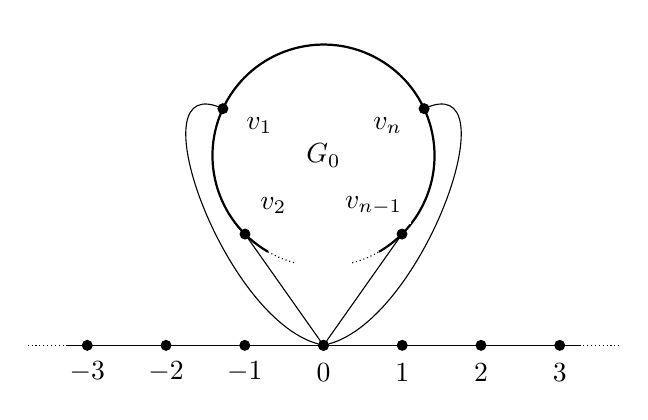
\begin{tikzpicture}[
  label distance=-5.5pt,
  thin,
  vertex/.style={circle,draw=black,fill=black,inner sep=1.25pt,
    minimum size =0mm},
  attach/.style={circle,draw=black,fill=white,inner sep=1.25pt,
    minimum size =0mm},
  dots/.style={circle,fill=black,inner sep=.5pt,
    minimum size= 0pt}]

% Path and Labels    
  \draw (-3.25,-2.41) -- (3.25,-2.41);
  
  \foreach \x in {-3,...,3}{
    \node at (\x,-2.41) [vertex] {};
    \node at (\x,-2.75) {$\x$};
  }
    
  \node (a) at (0,-2.41) [vertex] {};
  
  \draw[densely dotted] (-3.25,-2.41) -- (-3.75, -2.41);
  \draw[densely dotted] (3.25, -2.41) -- (3.75, -2.41);
  
% Graph  
  \draw[thick] (240:1.41) arc (240:-60:1.41);
  \draw[densely dotted] (240:1.41)  arc (240:255:1.41);
  \draw[densely dotted] (285:1.41)  arc (285:300:1.41);
  
  \foreach \i / \n /\t in {25 / n/ 15, 155 / 1/ 165, 225/ 2 / 120, 315 / {n-1}/60}{
    \node at (\i : .9) [rectangle,fill=white] {$v_\n$};
    \node at (\i : 1.41) [vertex] {};
  }
  \node at (0,0) [rectangle,fill=white] {$G_0$};

% Attaching Edges
  \foreach \i /\t in {25/15, 155/165}{
    \draw (\i:1.41) to[out=\i,in=\t] (a);
  }
  
  \foreach \i \in in {225,315}{
    \draw (\i:1.41) to (a);
  }

\end{tikzpicture}